\documentclass[journal,12pt,twocolumn]{IEEEtran}
\usepackage{setspace}
\usepackage{gensymb}
\singlespacing
\usepackage[cmex10]{amsmath}

\usepackage{amsthm}
\usepackage{hyperref}
\hypersetup{
    colorlinks=true,
    linkcolor=blue,
    filecolor=magenta,      
    urlcolor=cyan,
}

\urlstyle{same}
\usepackage{mathrsfs}
\usepackage{txfonts}
\usepackage{stfloats}
\usepackage{bm}
\usepackage{cite}
\usepackage{cases}
\usepackage{subfig}

\usepackage{longtable}
\usepackage{multirow}

\usepackage{enumitem}
\usepackage{mathtools}
\usepackage{steinmetz}
\usepackage{tikz}
\usepackage{circuitikz}
\usepackage{verbatim}
\usepackage{tfrupee}
\usepackage[breaklinks=true]{hyperref}
\usepackage{graphicx}
\usepackage{tkz-euclide}
\usetikzlibrary{shapes,backgrounds}
\usepackage{verbatim}
\usetikzlibrary{calc,math}
\usepackage{listings}
    \usepackage{color}                                            %%
    \usepackage{array}                                            %%
    \usepackage{longtable}                                        %%
    \usepackage{calc}                                             %%
    \usepackage{multirow}                                         %%
    \usepackage{hhline}                                           %%
    \usepackage{ifthen}                                           %%
    \usepackage{lscape}     
\usepackage{multicol}
\usepackage{chngcntr}
\usepackage{mdframed}
\DeclareMathOperator*{\Res}{Res}

\renewcommand\thesection{\arabic{section}}
\renewcommand\thesubsection{\thesection.\arabic{subsection}}
\renewcommand\thesubsubsection{\thesubsection.\arabic{subsubsection}}

\renewcommand\thesectiondis{\arabic{section}}
\renewcommand\thesubsectiondis{\thesectiondis.\arabic{subsection}}
\renewcommand\thesubsubsectiondis{\thesubsectiondis.\arabic{subsubsection}}


\hyphenation{op-tical net-works semi-conduc-tor}
\def\inputGnumericTable{}                                 %%

\lstset{
%language=C,
frame=single, 
breaklines=true,
columns=fullflexible
}

\usepackage{chngcntr}
\counterwithin{figure}{section}

\title{AI5002}
\author{TUHIN DUTTA}
\date{January 2021}

\begin{document}
\newtheorem{theorem}{Theorem}[section]
\newtheorem{problem}{Problem}
\newtheorem{proposition}{Proposition}[section]
\newtheorem{lemma}{Lemma}[section]
\newtheorem{corollary}[theorem]{Corollary}
\newtheorem{example}{Example}[section]
\newtheorem{definition}[problem]{Definition}

\newcommand{\BEQA}{\begin{eqnarray}}
\newcommand{\EEQA}{\end{eqnarray}}
\newcommand{\define}{\stackrel{\triangle}{=}}
\bibliographystyle{IEEEtran}
\raggedbottom
\setlength{\parindent}{0pt}
\providecommand{\mbf}{\mathbf}
\providecommand{\pr}[1]{\ensuremath{\Pr\left(#1\right)}}
\providecommand{\qfunc}[1]{\ensuremath{Q\left(#1\right)}}
\providecommand{\sbrak}[1]{\ensuremath{{}\left[#1\right]}}
\providecommand{\lsbrak}[1]{\ensuremath{{}\left[#1\right.}}
\providecommand{\rsbrak}[1]{\ensuremath{{}\left.#1\right]}}
\providecommand{\brak}[1]{\ensuremath{\left(#1\right)}}
\providecommand{\lbrak}[1]{\ensuremath{\left(#1\right.}}
\providecommand{\rbrak}[1]{\ensuremath{\left.#1\right)}}
\providecommand{\cbrak}[1]{\ensuremath{\left\{#1\right\}}}
\providecommand{\lcbrak}[1]{\ensuremath{\left\{#1\right.}}
\providecommand{\rcbrak}[1]{\ensuremath{\left.#1\right\}}}
\theoremstyle{remark}
\newtheorem{rem}{Remark}
\newcommand{\sgn}{\mathop{\mathrm{sgn}}}

\providecommand{\res}[1]{\Res\displaylimits_{#1}} 

%\providecommand{\norm}[1]{\lVert#1\rVert}
\providecommand{\mtx}[1]{\mathbf{#1}}
\providecommand{\fourier}{\overset{\mathcal{F}}{ \rightleftharpoons}}
%\providecommand{\hilbert}{\overset{\mathcal{H}}{ \rightleftharpoons}}
\providecommand{\system}{\overset{\mathcal{H}}{ \longleftrightarrow}}
	%\newcommand{\solution}[2]{\textbf{Solution:}{#1}}
\newcommand{\solution}{\noindent \textbf{Solution: }}
\newcommand{\cosec}{\,\text{cosec}\,}
\providecommand{\dec}[2]{\ensuremath{\overset{#1}{\underset{#2}{\gtrless}}}}
\newcommand{\myvec}[1]{\ensuremath{\begin{pmatrix}#1\end{pmatrix}}}
\newcommand{\mydet}[1]{\ensuremath{\begin{vmatrix}#1\end{vmatrix}}}
\numberwithin{equation}{subsection}
\makeatletter
\@addtoreset{figure}{problem}
\makeatother
\let\StandardTheFigure\thefigure
\let\vec\mathbf
\renewcommand{\thefigure}{\theproblem}
\def\putbox#1#2#3{\makebox[0in][l]{\makebox[#1][l]{}\raisebox{\baselineskip}[0in][0in]{\raisebox{#2}[0in][0in]{#3}}}}
     \def\rightbox#1{\makebox[0in][r]{#1}}
     \def\centbox#1{\makebox[0in]{#1}}
     \def\topbox#1{\raisebox{-\baselineskip}[0in][0in]{#1}}
     \def\midbox#1{\raisebox{-0.5\baselineskip}[0in][0in]{#1}}
\vspace{3cm}
\title{AI5002 - Assignment 11}
\author{Tuhin Dutta\\ ai21mtech02002}
\maketitle
\newpage
\bigskip
\renewcommand{\thefigure}{\theenumi}
\renewcommand{\thetable}{\theenumi}
\begin{mdframed}
Download code and LaTeX from below hyperlinks\\
1. \href{https://github.com/Tauhait/AI5002/blob/main/Assignment-11/Code/GATE_13.py}{Code/GATE\_13.py}


2. \href{https://github.com/Tauhait/AI5002/tree/main/Assignment-11/LaTeX}{LaTeX}
\end{mdframed}
\subsection*{\boldsymbol{Problem\ GATE13}}
Two players, A and B, alternately keep rolling a fair dice. The person to get a six first wins the game. Given that player A starts the game, the probability that A wins the game is ...\\
\\
(\text{A})\ \dfrac{5}{11}\ \ \ \ \ \ (\text{B})\ \dfrac{1}{2}\ \ \ \ \ \ (\text{C})\ \dfrac{7}{13}\ \ \ \ \ \ (\text{D})\ \dfrac{6}{11}\ \ \ \ \ \
\subsection*{\boldsymbol{Solution}}
Let us define a r.v. X.
\begin{align}\tag{1.01}
    \begin{split}
        X &= \{\text{`Odd \# trial to get six by A'}\}.\\
          &= \{\ 1, 3, 5, 7, ...\ \}
    \end{split}
\end{align}
Probability of throwing a die to get 6.
\begin{equation}\tag{1.02}
\begin{split}
    Pr\ & \Big(p=\text{`Getting a 6'}\Big) = \dfrac{1}{6}\\
    Pr\ & \Big((1-p)=\text{`Getting a non 6'}\Big) = \dfrac{5}{6}
\end{split}
\end{equation}
The probability distribution of X is geometric.
\begin{align}\tag{1.03}
    X \sim Geo\ \Big(p\Big)
\end{align}
Probability of first six thrown by A in the k$^{th}$ odd trial to win the game - 
\begin{align}\tag{1.04}
    \pr{X = k} = (1-p)^{k-1}.p
\end{align}
for k = 1, 2, 3, ....\\
\\
Getting a six in the 1$^{st}$ trial thrown by A
\begin{align}\tag{1.05}
    \pr{X = 1} = (1-p)^{0}.p = \Big(\dfrac{5}{6}\Big)^{0}.\dfrac{1}{6}
\end{align}
Getting a six in the 3$^{rd}$ trial thrown by A
\begin{align}\tag{1.06}
    \pr{X = 3} = (1-p)^{2}.p = \Big(\dfrac{5}{6}\Big)^{2}.\dfrac{1}{6}
\end{align}
Getting a six in the 5$^{th}$ trial thrown by A 
\begin{align}\tag{1.07}
    \pr{X = 5} = (1-p)^{4}.p = \Big(\dfrac{5}{6}\Big)^{4}.\dfrac{1}{6}
\end{align}
Getting a six in the 7$^{th}$ trial thrown by A 
\begin{align}\tag{1.08}
    \pr{X = 7} = (1-p)^{6}.p = \Big(\dfrac{5}{6}\Big)^{6}.\dfrac{1}{6}
\end{align}
\begin{align*}
    \vdots
\end{align*}
Probability that A wins the game
\begin{align}\tag{1.09}
\begin{split}
    \pr{Y=\text{`A wins the game'}} = \pr{X=1}\ + \pr{X=3}\ +\\ \pr{X=5}\ + \pr{X=7}\ +\\ \cdots
\end{split}
\end{align}
\begin{align}\tag{1.10}
    \begin{split}
        \pr{Y=\text{`A wins the game'}} = \dfrac{1}{6}\ +\ \Big(\dfrac{5}{6}\Big)^{2}.\dfrac{1}{6}\ + \Big(\dfrac{5}{6}\Big)^{4}.\dfrac{1}{6}\ +\\ \ \Big(\dfrac{5}{6}\Big)^{6}.\dfrac{1}{6}\ +\\ \ \cdots 
    \end{split}
\end{align}

From (1.10), we compare it to a infinite geometric sequence as below,\\
\begin{equation}\tag{1.11}
    \begin{split}
        s = ar^0 + ar^1 + ar^2 + ar^3 + ar^4 + \cdots
    \end{split}
\end{equation}
The first term and common ratio of (1.11) is given by - 
\begin{equation}\tag{1.11}
    \begin{split}
        a &= \dfrac{1}{6}
        \\
        \\
        r &= \Big(\dfrac{5}{6}\Big)^{2}, \ \ 0 \leq r \leq 1
    \end{split}
\end{equation}
The closed form summation of (1.11) is given by \\
\begin{equation}\tag{1.12}
    \begin{split}
        s &= \dfrac{a}{1 - r}\\
    \end{split}
\end{equation}
From (1.12), on substituting values, we get
\begin{equation}\tag{1.13}
    \begin{split}
        s &= \dfrac{\dfrac{1}{6}}{1 - \dfrac{25}{36}} = \dfrac{\dfrac{1}{6}}{\dfrac{11}{36}}\\
          &= \dfrac{6}{11}
    \end{split}
\end{equation}
\begin{figure}[h!]
    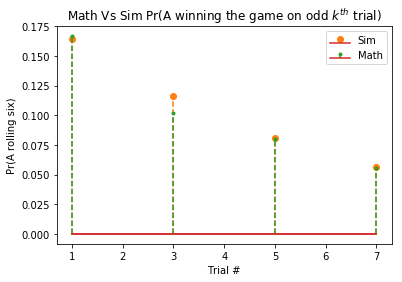
\includegraphics[width=10cm]{Assignment-11/Code/Figure/plot.png}
\end{figure}
\end{document}
